% \iffalse meta-comment
%
% Copyright 2000-2001
% Karsten Tinnefeld <karsten@tinnefeld.com>
%
% -----------------------------------------
% This file is part of the bophook package,
% a contribution to the LaTeX2e system. 
% -----------------------------------------
%
% It may be distributed and/or modified under the conditions of the 
% LaTeX Project Public License, either version 1.2 of this licence, or
% (at your option) any later version. The latest version of this license
% is in http://www.latex-project.org/lppl.txt and version 1.2 is part
% of all distributions of LaTeX version 1999/12/01 or later.
%
%  This program consists of bophook.dtx and bophook.ins.
%
\NeedsTeXFormat{LaTeX2e}
%<*dtx>
\ProvidesFile{bophook.dtx}
%</dtx>
%<!driver>\ProvidesPackage{bophook}
%<driver>\ProvidesFile{bophook.drv}
% \fi
% \ProvidesFile{bophook.dtx}
  [2001/03/29 v0.02 beginning-of-page hook, K. Tinnefeld]
% \iffalse
%<*driver>
\documentclass{ltxdoc}
\usepackage{multicol}
\GetFileInfo{bophook.dtx}
\newcommand*{\docdate}{2001/03/29}
\EnableCrossrefs
%\DisableCrossrefs% when index is ready
\CodelineIndex
\RecordChanges
\def\example{Re-run \LaTeX\ on the documentation after installing
  {\MacroFont bophook.sty} in order to see an example of this.}
\IfFileExists{bophook.sty}{%
  \RequirePackage{bophook}
  \AtBeginPage{%
    \setlength{\unitlength}{1cm}
    \put(3, -5){\makebox(0,0)[tl]{\framebox{image}}}}
  \def\example{This page has a box created according to these
    parameters.}}{}
\begin{document}
  \DocInput{bophook.dtx}
\end{document}
%</driver>
% \fi
%
% \CheckSum{99}
%
% \changes{v0.01}{2000/03/07}{Initial Revision (KT).}
% \changes{v0.02}{2001/03/29}{Adaptation for use with hyperref (KT).}
%
%  \DoNotIndex{\@empty, \@begindvibox, \box, \CheckCommand, \dp,
%  \else, \fi, \gdef, \global, \hb@xt@, \hss, \@ifpackageloaded,
%  \ignorespaces, \let, \moveleft, \newcommand, \renewcommand, \relax,
%  \setbox, \unvbox, \vbox, \vskip, \vss, \z@, \ProcessOptions}
%
% \date{printed \today}
% \title{\texttt{bophook}, a beginning-of-page hook\thanks{This file
%   has version number \fileversion, last revised on \filedate,
%   documentation dated \docdate.}}
% \author{Karsten Tinnefeld\\
%         Universit\"at Dortmund\\
%         \texttt{karsten@tinnefeld.com}}
% \maketitle
%
%  \section{Introduction}
%  This program adds two \LaTeX\ hooks to set up the page layout and
%  output material in the background of every page.  In order to use
%  the package with |hyperref|, you have to load |hyperref| first.
%
%  \DescribeMacro{\AtBeginPage} Using the |\AtBeginPage| hook, you can
%  add material in the background of a page.  Think of it as a
%  construct that does:  For every page, create a picture environment
%  with its origin at the top left corner\footnote{When I mean the top
%  left corner or the paper, I do \emph{not} mean some 25.4mm down and
%  to the right of it.} of the paper (resp., output device).  So for
%  example, you can put an image that is three centimeters from the
%  left border and five from the top border by 
%  saying\footnote{\example}
%  \begin{verbatim}
%    \AtBeginPage{%
%      \setlength{\unitlength}{1cm}
%      \put(3, -5){\makebox(0,0)[tl]{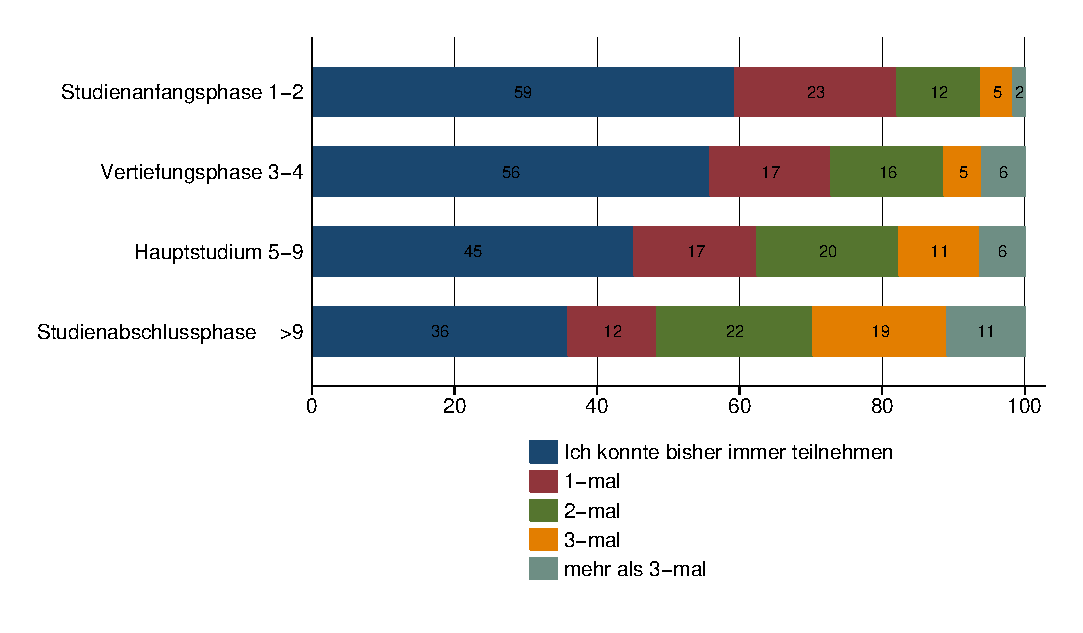
\includegraphics{image}}}}
%  \end{verbatim}
%
%  Of course, reusing |\AtBeginPage| during the document changes the
%  page background of the next page that is going to start.  No
%  spurious spaces are generated whatsoever. |\AtBeginPage| eats up
%  every white space after its closing brace to allow its use in
%  horizontal mode.  This hook uses normal \TeX\ boxes and is
%  therefore not bound with respect to a certain output driver.
%
%  \DescribeMacro{\PageLayout} In normal \LaTeX\ page makeup, there is
%  few if any room for a user to re-define page width and length
%  and/or margin settings.  These should be set in the |\ps@...|
%  commands, but are sometimes interfering with current pages that
%  have not yet been shipped out.  The idea is that a page style
%  command should give these makeup commands wrapped in
%  |\PageLayout{}|, which is guaranteed to be executed on every page
%  where that page style is in effect.
%
%  \StopEventually {}
%
%  \section{Realization}
%  We straightforwardly modify the output routine where
%  the |\AtBeginDvi| code takes place.  This could clash with any
%  other routine that does the same thing.  Caveat emptor.
%
%  Start by ignoring all options.
%
%    \begin{macrocode}
\ProcessOptions \relax
%    \end{macrocode}
%
%  \begin{macro}{\PageLayout}
%    The |\PageLayout| command just stores its argument in a global
%    variable, which is initialized with the empty value.
%    \begin{macrocode}
\newcommand*{\PageLayout}[1]{\gdef\BH@pagelayout{#1}\ignorespaces }
\let \BH@pagelayout \relax
%    \end{macrocode}
%  \end{macro}
%
%  \begin{macro}{\AtBeginPage}
%    Likewise does |\AtBeginPage|.
%    \begin{macrocode}
\newcommand*{\AtBeginPage}[1]{\gdef\BH@originpic{#1}\ignorespaces }
\let \BH@originpic \relax
%    \end{macrocode}
%  \end{macro}
%
%  The |hyperref| package does a lot of modification to the \LaTeX\
%  kernel.  Prepare for the case that it is loaded.  Note that it has
%  to be loaded prior to |bophook|!
%
%  We check the original definition of the internal begin-dvi hook.
%  In case this has been modified, either by a new kernel or another
%  style file, a warning will be issued.
%
%    \begin{macrocode}
\@ifpackageloaded{hyperref}{%
  \CheckCommand*\@begindvi{%
    \unvbox \@begindvibox
    \ifHy@pageanchor
      \@hyperfixhead
      \global\let \@begindvi \@hyperfixhead
      \else
      \global\let \@begindvi \HyPL@EveryPage
    \fi }}{%
  \CheckCommand*\@begindvi{%
    \unvbox \@begindvibox
    \global\let \@begindvi \@empty}}
%    \end{macrocode}
%
%  \begin{macro}{\@begindvi}
%    Having verified, that it is like it should have been, we insert
%    our own code.  |\AtBeginDvi|-code is still executed on the first
%    page before the |\AtBeginPage|-code of page~1.  No provision is
%    taken (as it was) that |\AtBeginDvi|-code might create typeset
%    output.
%
%    |hyperref| performs different actions according to a switch.
%    This behaviour is initiated at the start of the first page.  We
%    record it for reference in |\@BH@originpic|.
%
%    \begin{macrocode}
\let \BH@hyperpageaction \@empty
\@ifpackageloaded{hyperref}{%
  \renewcommand*\@begindvi{%
    \unvbox \@begindvibox
    \ifHy@pageanchor
      \@hyperfixhead
      \BH@originprint
      \global\let \BH@hyperpageaction \@hyperfixhead
      \else
      \BH@originprint
      \global\let \BH@hyperpageaction \HyPL@EveryPage
    \fi
    \global\let \@begindvi \BH@originprint
    }}{% no hyperref
  \renewcommand*\@begindvi{%
    \unvbox \@begindvibox
    \BH@originprint
    \global\let \@begindvi \BH@originprint}}
%    \end{macrocode}
%  \end{macro}
%
%  \begin{macro}{\BH@originprint}
%    We create a box that will be inserted at the ``page origin'' in
%    the arcane Knuthian sense, that is, one inch down and to the
%    right of the output medium start. It consists of the move to the
%    real origin and the formatting of the |\AtBeginPage|-code flush
%    top left and taking no horizontal nor vertical space.  As one can
%    easily see from the documentation of the |picture|-environment,
%    there is no magic about a |picture|---a |\put|-command can simply
%    be issued everywhere.  It is however well sensible to
%    \emph{interprete} the typeset material as a |picture|.
%
%    \begin{macrocode}
\newcommand*{\BH@originprint}{%
  \setbox\@tempboxa\vbox to\z@{%
    \vskip-1in \moveleft1in \vbox{%
      \hb@xt@\z@{%
        \BH@originpic\hss}}\vss}
  \dp\@tempboxa\z@
  \box\@tempboxa \BH@pagelayout
  \BH@hyperpageaction }
%    \end{macrocode}
%  \end{macro}
%
%\Finale
%
%% \CharacterTable
%%  {Upper-case    \A\B\C\D\E\F\G\H\I\J\K\L\M\N\O\P\Q\R\S\T\U\V\W\X\Y\Z
%%   Lower-case    \a\b\c\d\e\f\g\h\i\j\k\l\m\n\o\p\q\r\s\t\u\v\w\x\y\z
%%   Digits        \0\1\2\3\4\5\6\7\8\9
%%   Exclamation   \!     Double quote  \"     Hash (number) \#
%%   Dollar        \$     Percent       \%     Ampersand     \&
%%   Acute accent  \'     Left paren    \(     Right paren   \)
%%   Asterisk      \*     Plus          \+     Comma         \,
%%   Minus         \-     Point         \.     Solidus       \/
%%   Colon         \:     Semicolon     \;     Less than     \<
%%   Equals        \=     Greater than  \>     Question mark \?
%%   Commercial at \@     Left bracket  \[     Backslash     \\
%%   Right bracket \]     Circumflex    \^     Underscore    \_
%%   Grave accent  \`     Left brace    \{     Vertical bar  \|
%%   Right brace   \}     Tilde         \~}
%
%\endinput
